%\KOMAoptions{paper=landscape,pagesize}
\recalctypearea

\Large \textbf{\center{Appendix}} \normalsize
\raggedright

%\setcounter{page}{1}
%\renewcommand{\thepage}{A\arabic{page}}

\setcounter{figure}{0}
\renewcommand{\thefigure}{A\arabic{figure}}

\setcounter{table}{0}
\renewcommand{\thetable}{A\arabic{table}}

\setcounter{section}{0}

\section{Facebook vs Non-Facebook Sampling}
\subsection{Outreach via Web Scraping Emails}
We employed several different strategies to recruit companies to obtain a diverse and representative sample of managers. We found some methods, particularly targeted Facebook ads, to be far more effective than others. As discussed in our pre-registration, our initial sampling strategy involved collecting a substantial number of email addresses of a cross-section of U.S. firms. We were interested in hearing from all firms and not just the larger publicly-traded companies with established government relations practices. To do so, we began with a random sample of all U.S. firms in the Orbis database, and then used web crawling techniques to identify email addresses. Orbis data reflects the pattern of business establishment in the U.S., meaning that the vast majority of firms represented are small (under 5 employees) and concentrated in the services sector (ex. retail, professional services, transportation, leisure and hospitality etc). This sample is appropriate because firms of all sizes and all along the supply chain, including non-tradable firms, could potentially experience tariffs if they use any tradable input. For example, housing construction is non-tradable but the steel, aluminum, and lumber used are exposed to tariffs. 

However, we found this sampling method to be impractical because of aggressive spam filters and the deluge of questionable emails that business managers receive. For this initial wave during June 2019, we reached out to over 12,000 firms by email and only received 2 survey responses or 0.017 percent. Many of the emails generated by web crawling were general inquiry info@companyname.com rather than personal email addresses. After sending out a reminder email and receiving more angry requests to stop spamming respondents than actual survey responses, we changed our outreach strategy. 
\subsection{Outreach via Phone and Email}
From August 2019 to March 2020, we assigned research assistants to manually look up the emails and phone numbers of managers, introduce the survey, and solicit for a manager's personal email to send the survey instrument. The Orbis sample was divided into time zones and we hired Upworkers to help gather manager emails. We learned quickly that undergraduate research assistants were much more effective than Upworkers. So we hired teams of research assistants at the University of Kansas and Brigham Young University worked off of the Orbis sample to call businesses during their regular business hours. Students were also given a script to ask the first ten questions of the survey over the phone rather but we still needed to follow up by sending the survey instrument by email to give the treatment. 

The teams manually checked a total of 6149 firms from the Orbis sample and found a total of 3447 phone numbers. 1516 calls were made using these phone numbers and the response rate was 56 percent, the other 44 percent of numbers were either disconnected or went to an automated phone system. We judge that the phone-call-collected manager emails are likely the most reliable and up-to-date, and given that they also assented to taking a survey, those emails were given highest priority. However, many employees and managers refused to participate and the team was only able to obtain 120 valid emails. These phone conversations yielded 46 partial or complete responses. The completion rate is significantly higher than web scraping emails but still pretty low at 0.75 percent. The onset of the pandemic and the high costs of this approach led us to adjust strategy yet again with two parallel efforts.  

\subsection{Outreach via Purchased Emails}
In June 2020, we contracted the services of FrescoData, a marketing company. They promised to email their proprietary list of 25,000 managers three times for \$4000. We asked them to split the sample into control and treatment. The company estimated successful delivery rate to be 97 percent, the open rate was estimated to be 24-29 percent, and the click rate was supposed to be 6-9 percent. We expected 1500 or so responses overall but only recorded 2 partial responses, a 0.008 completion rate.    

\subsection{Outreach via Kansas City Chamber of Commerce}
In January 2020, we negotiated a partnership with the Kansas City Chamber of Commerce (KC Chamber) and the affiliated World Trade Center KC (WTC-KC). The KC Chamber has over 2200 members in the greater Kansas City metro area, spread across 14 counties in Kansas and Missouri. 90 percent of KC Chamber members are defined as small businesses with fewer than 250 full time employees. But the KC Chamber also includes some bigger multinational companies with thousands of employees like Hallmark, H\&R Block, Garmin, Cerner, and Commerce Bank as well as subsidiaries of Fortune 500 companies such as FedEx, Honeywell, PNC Bank, T-Mobile (Sprint), and Bayer (Crop Sciences). The WTC-KC is the international arm of the KC Chamber and the local chapter of the World Trade Centers Association. Its mission is to help local businesses engage in global commerce. The KC Chamber agreed to help us market the survey to its members in exchange for Dr. Jack Zhang presenting the preliminary results of our survey at the Go Global KC 2020 event and for the purchase of 10 Go Global KC tickets to raffle off as prizes. Between May and June of 2020, the KC Chamber advertised the survey in its newsletter and on its facebook page. We also tasked a team of University of Kansas students and WTC-KC interns to draft personalized messages to 570 subscribers to the WTC-KC international trade mailing list, firms we believe are the most likely to be exposed to tariffs. These waves of outreach yielded 66 valid responses, a 3 percent completion rate.  

\begin{figure}
    \centering
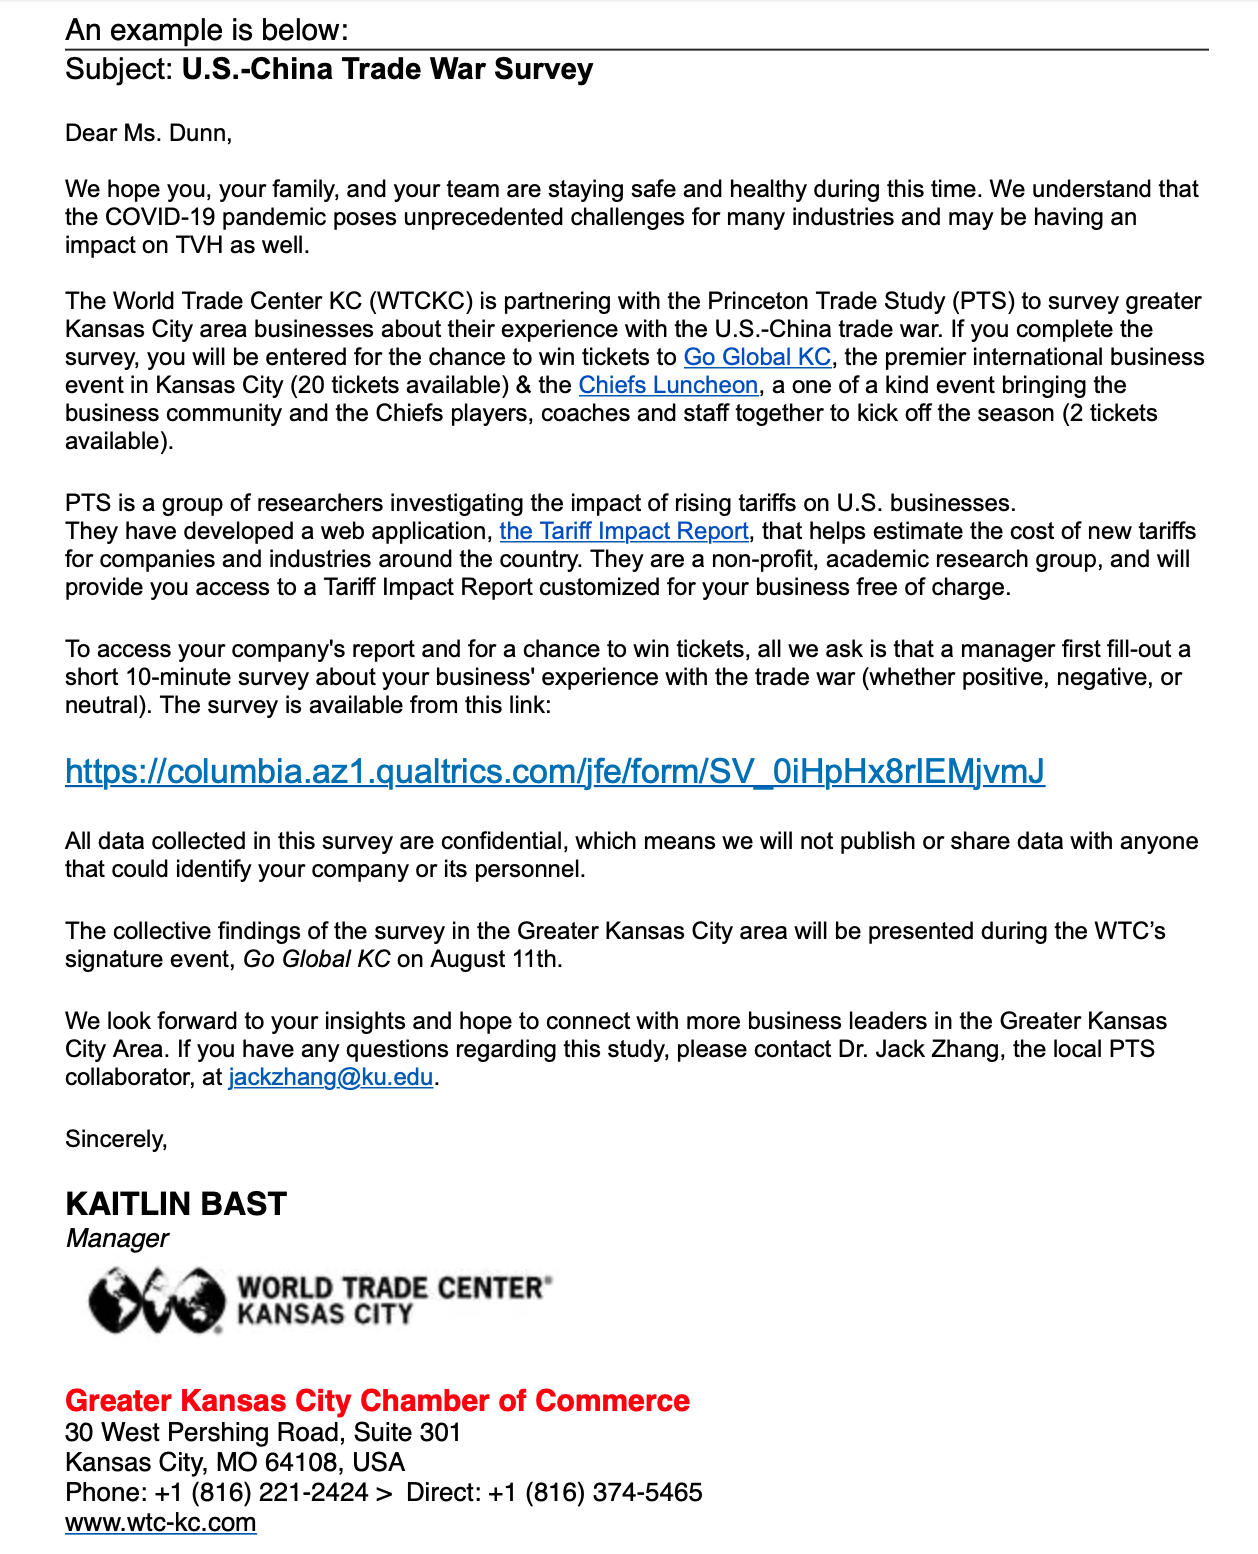
\includegraphics[scale=.5]{KC chamber email.png}
    \caption{Sample Personalized Email from KC Chamber}
    \label{fig:kcchamber}
\end{figure}

\subsection{Outreach via Targeted Facebook Ads}

Targeted ads on Facebook proved to be our most effective sampling strategy. During 2019, we also experimented with contacting managers through Twitter or LinkedIn but found Facebook to be the most cost-effective. We paid to target ads at managers in the United States. We ran two rounds of targets ads on Facebook in June 2019 and July 2020. 

We over-incentivized the first round of sampling by offering a \$5 gift Amazon card. A large number of participants lied about being a manager in order to obtain the reward. We describe below the methods we used to cull the 1747 responses obtained from this wave down to 603 valid responses. We also ran a second round of ads without any incentives one year later, after the Phase One Trade Deal was signed and the onset of the COVID-19 pandemic exacerbated supply chain issues. This wave yielded 335 valid responses. It is hard to calculate a comparable completion rate for the Facebook sample. But we calculate it to be 938 responses from 100,000? impressions. This is a comparably low completion rate as the validated email outreach but much more cost effective.    

\subsection{Validation of Facebook Sample}

Research assistants at the University of Kansas and Wesleyan University helped devise a system for detecting suspicious responses from the Facebook sample based on total response time, IP addresses, and verifying the business name or manager email. The criteria for whether or not a response was invalid are as follows (need two hits to be deemed invalid): 

1) \textit{total response time} - flagged responses under 120s as having a high probability of professional survey taker. Some justification for this: the non-facebook sample had a median response time of 375s, the invalid Facebook responses had a median of 188s. Removing these the Facebook sample has a median response time of 261s 

2) \textit{googling the business name or follow up email} - our RAs did a really good and through job, here are some of my favorite notes: 
- Followed up by e-mail and she is a part-time cannabis trimmer 
- Blogger. in her words "I am not a professional nail artist or anything, it's just a hobby.”
- Facebook page is clearly one baking student
- Domain name is porn
- Reposts where to answer surveys for cash 

3) \textit{identifying duplicate or suspicious IP addresses} - many of the multiple IP hits came from Brazil, Mexico, Venezuela, Australia, these are flagged as invalid 

After applying this screening process, we ended up with 603 valid responses. 
Invalid: 576 responses - flagged for two or more reasons 
Maybe: 568 responses - unable to verify information, usually because no email was provided OR not employed at a business (ex. School, church, non-profit) 
Valid: 603 responses - basically anyone who is real and not trying to scam us: includes not manger, includes many one person "businesses"

The median response time for the valid Facebook sample is 261 seconds compared to 375 seconds for the non-Facebook sample (Email, Phone, KC Chamber). The median size of the valid Facebook sample is 8 employees, the mean is 3160. The median size of the non-facebook sample is 7 employees, and the mean is 7539. The median tariff impact (hurt\_trade) of the valid Facebook sample is 5 (neither), the mean is 4.45 (somewhat harmed). The median tariff impact of the non-facebook sample is 4 (somewhat harmed), the mean is 3.85. This is very promising and suggests that the two are comparable for external validity purposes.  

%Non-facebook sample: 136 
%Orbis Email blast: 2 
%Orbis Phone sample: 68 
%KC Chamber Email + Social Media: 66
%Median response time: 375 seconds 

%Facebook sample: ~605-653
%Median response time: 261 seconds (drop invalids, median of 188s) 


\section{Calculating Industry-Specific Costs of Tariffs}

Our goal was to estimate the costs of the trade war for a highly specific industry.

We began by creating an index of all the unique industries we wanted to generate estimates for. In the original version of our project, our sample was to be a random sample of all firms in Orbis. Even though we ended up pivoting to a primarily Facebook sample, the random sample from Orbis provided the original index of industries we estimated tariff costs for. Our Orbis sample was so large that we caught most industries using this approach. Only about 10\% of our Facebook sample provided an industry for which we were missing estimates.

Next, we wished to identify the input industries to each industry represented in the Orbis data. To do this, we turned to the Bureau of Economic Analysis Input-Output Use Table from 2012.\footnote{Available at \url{https://www.bea.gov/industry/input-output-accounts-data}.} (As of 2019, 2012 was the most recently available year for a widespread group of industries.) The Use tables provide, for every industry, the quantity that industry uses from other industries (see Figure \ref{fig:bea}).

\begin{figure}
    \centering
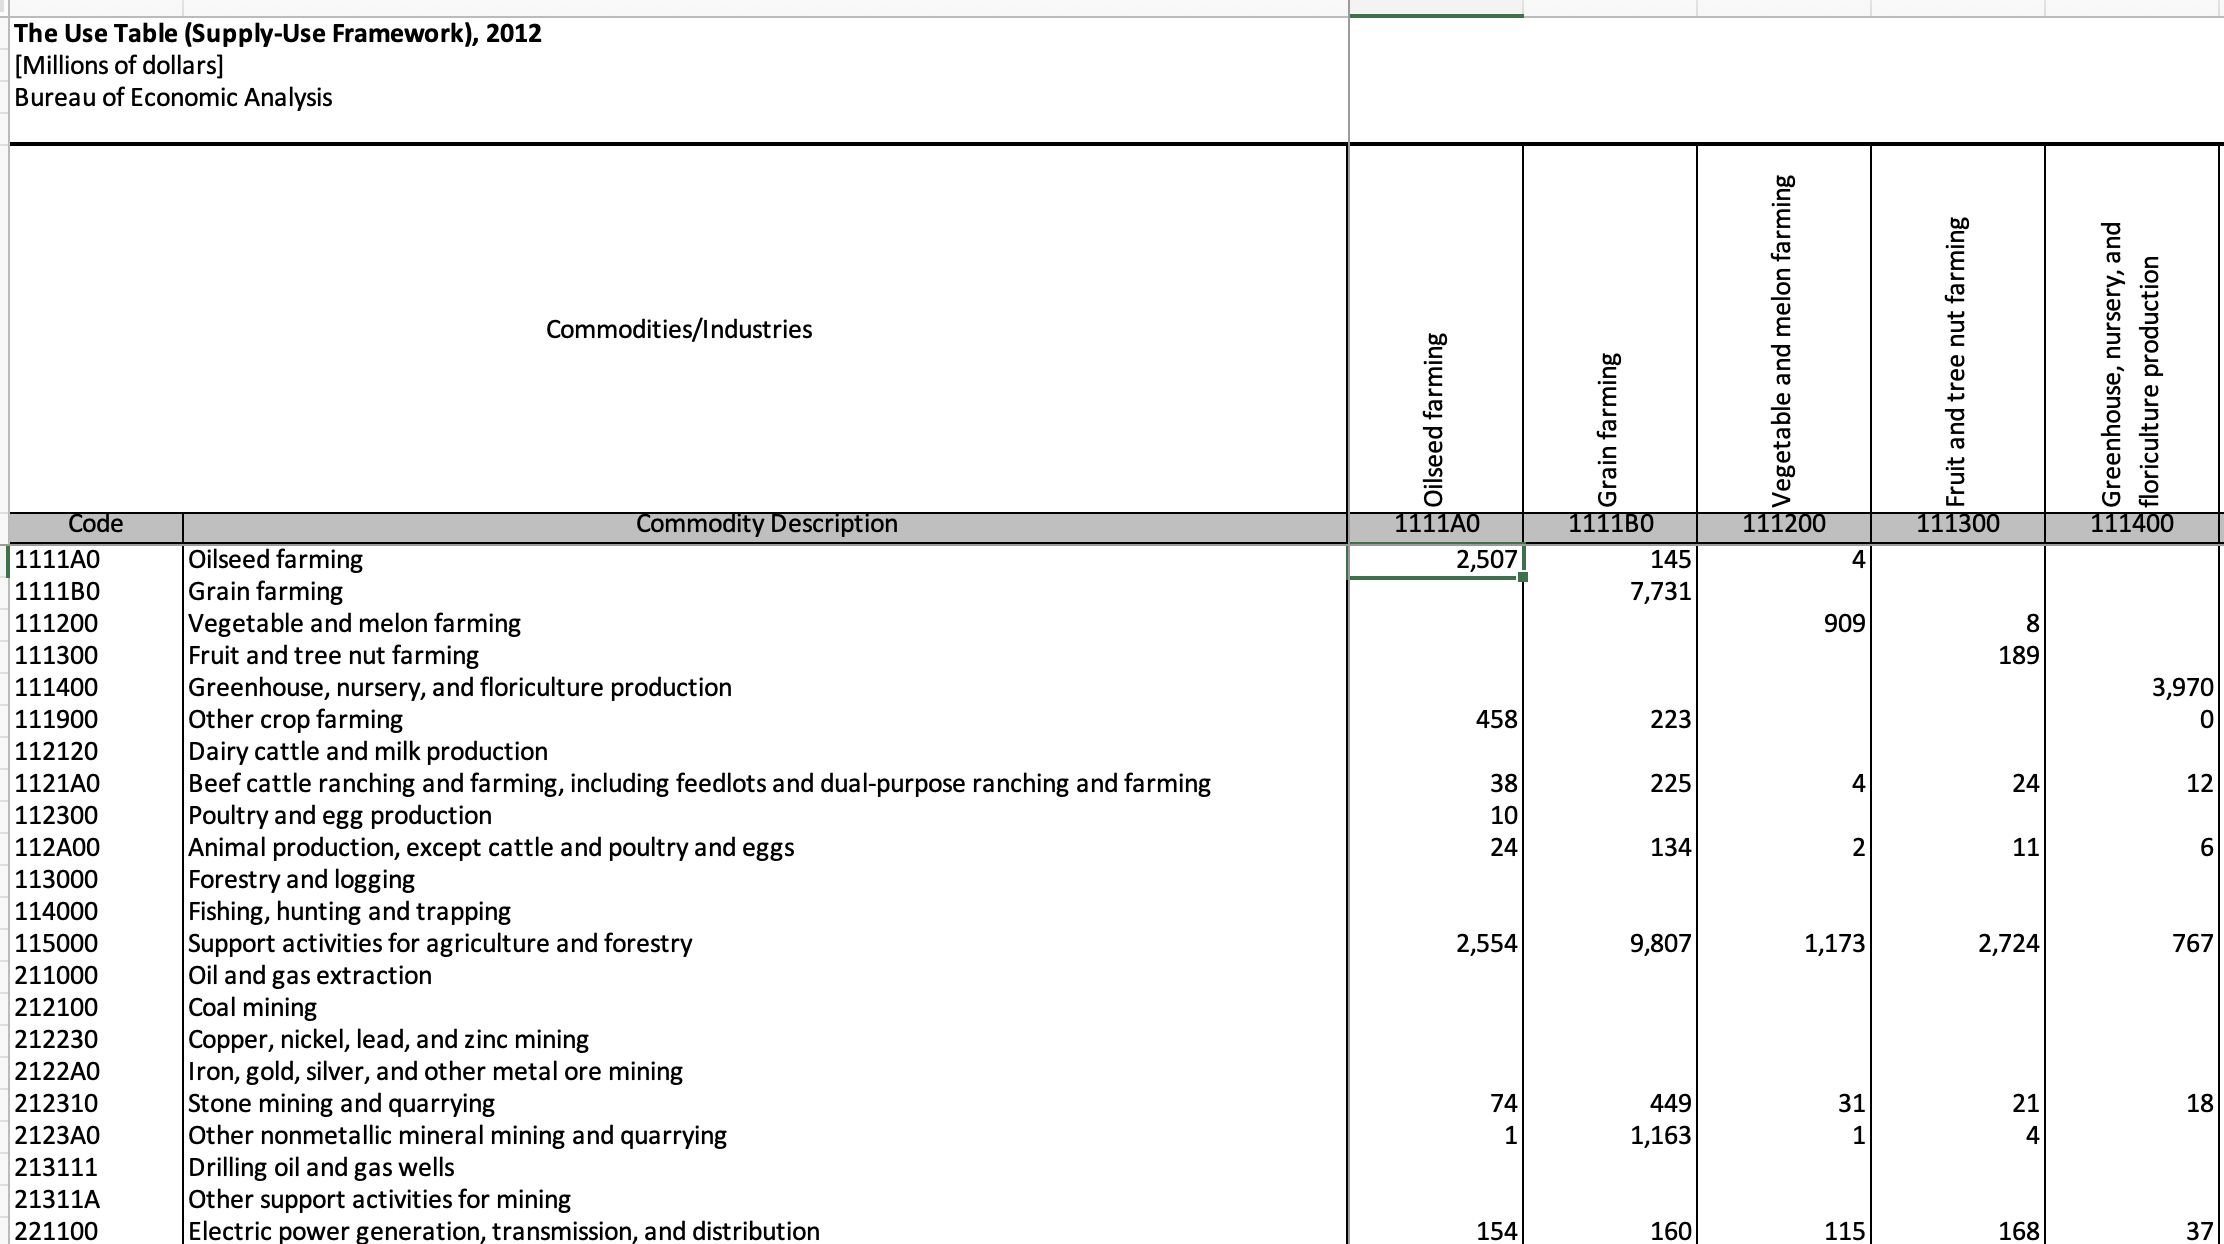
\includegraphics[scale=.4]{bea.png}
    \caption{BEA Use Table}
    \label{fig:bea}
\end{figure}

We merged the NAICS codes from Orbis and the NAICS codes from the BEA at the 3-digit level. This resulted in matches for 94\% of the industries from the Orbis data. When we merged at the 6-digit level, we found matches for only 17\% of the industries from the Orbis data. Since we merged at the 3-digit level, we aggregated the quantities from input industries as reported in the BEA for each 3-digit industry.

Once we knew which input industries each industry relied on, we wanted to know which commodities were associated with each input industry. We did this using a concordance from \cite{pierce2009concording}.\footnote{Available at \url{http://faculty.som.yale.edu/peterschott/sub_international.htm}.} The concordance identifies for each industry (6-digit NAICS) the various commodities associated with that industry (HTS codes) (see Figure \ref{fig:concordance}. We aggregate industries to the 3-digit level to merge with our previous data.

\begin{figure}
    \centering
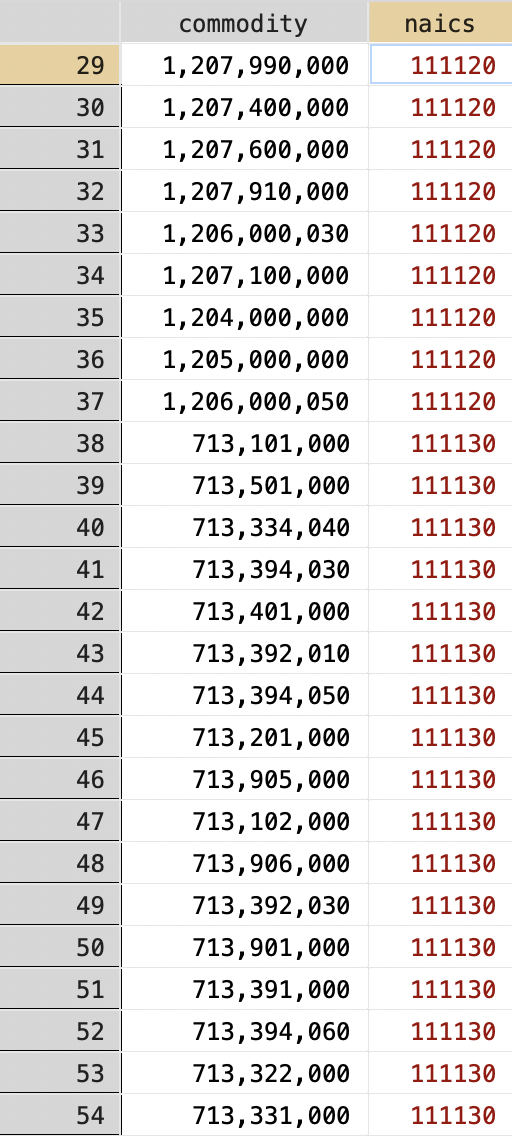
\includegraphics[scale=.4]{concordance.png}
    \caption{Concordance from Pierce and Schott (2009)}
    \label{fig:concordance}
\end{figure}

Last, we wanted to know whether each commodity associated with an input industry was subject to a tariff. We used data made available by Chad Bown at the Peterson Institute for International Economics.\footnote{Available at \url{https://piie.com/system/files/documents/bown2019-02-14.zip}.} An example appears in Figure \ref{fig:bown}. The data indicate which of the various tariff lists each commodity appears on (1) or does not appear on (0).

\begin{figure}
    \centering
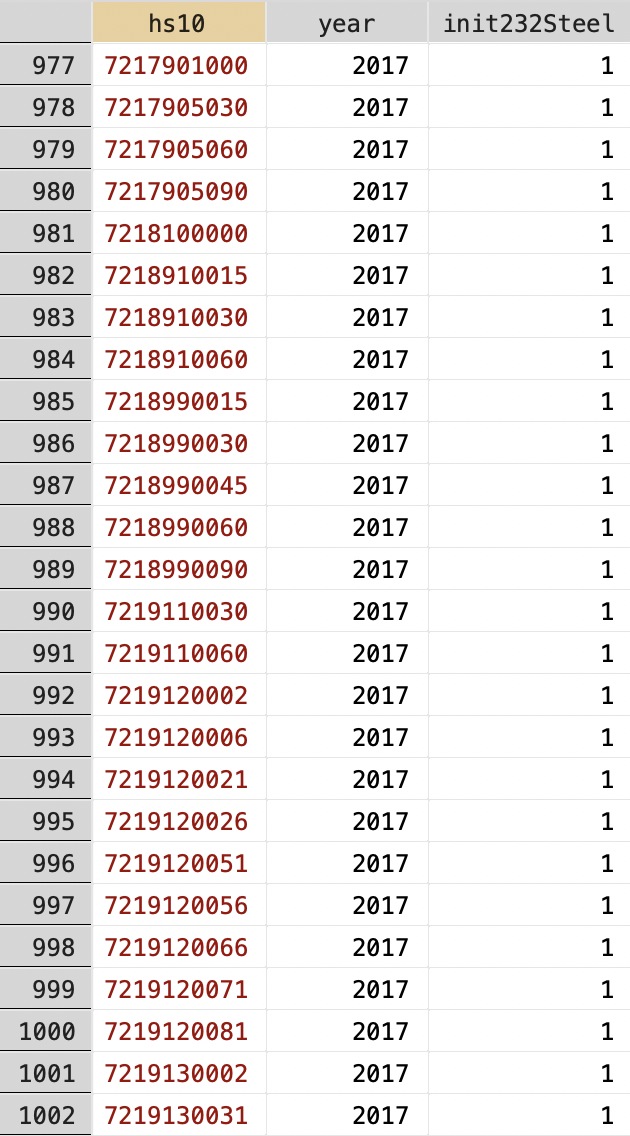
\includegraphics[scale=.4]{bown.png}
    \caption{Tariff Lists from Bown and Zhang}
    \label{fig:bown}
\end{figure}

These data allowed us to estimate, for each input industry, how many commodities it was associated with, how many of those commodities appeared on tariff lists, and the average tariff rate of the lists its commodities appear on. As we explain in the main paper, we summarize this to respondents as the number of tariffed products, the proportion of tariffed products, and the average tariff rate.

We did not want to overwhelm respondents with information, and we did want to provide them with information that would encourage them to act to oppose the trade war. For these reasons, we chose to share with respondents the estimates for the input industries that had the highest proportion of tariffed products (Figure \ref{fig:treatment_pic}). We ordered them first according the highest proportion of tariffed products and second according to which input industries were of greatest value to the industry in question.

\begin{figure}
    \centering
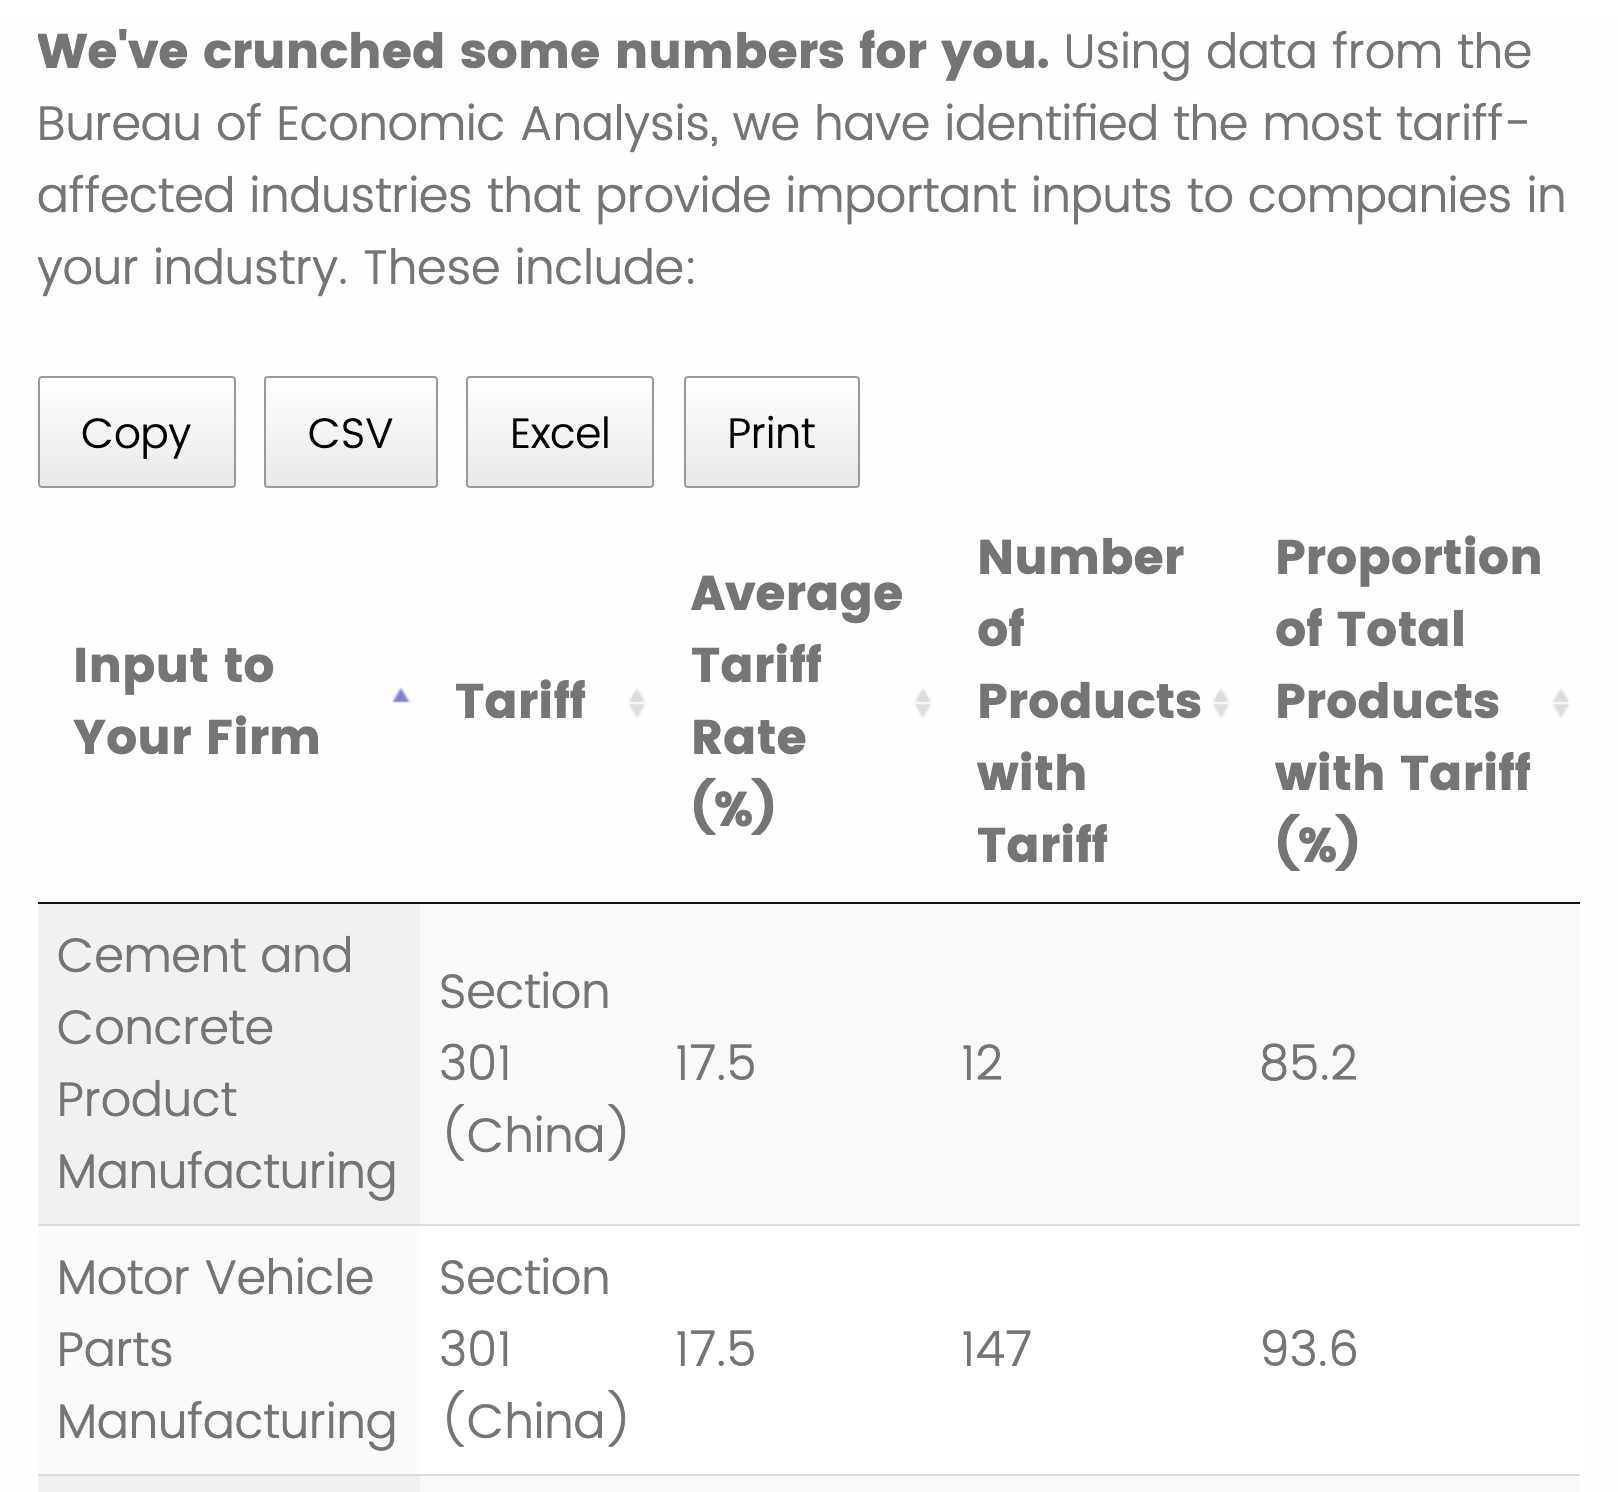
\includegraphics[scale=.4]{treatment_pic.png}
    \caption{Example of Static Treatment}
    \label{fig:treatment_pic}
\end{figure}

\section{ATEs for Support Trade War Outcomes}

In this section we include supplementary results for our support for the trade war outcome, along with a different operationalization of the outcome that looks at the count of outcomes for support or oppose was selected versus whether any one outcome was selected.

\input{tables/all_supp}
\input{tables/collapse_supp}
\input{tables/count_mods}

\section{Model Coefficients for Curvilinear Interactions}

In this section we show the underlying model results for Figures 4 and 5 in the main text.

\input{tables/out_mod_curv}

\section{Model Results for Number of Tariffs Shown}

In this section we report the full model results for our models estimating the effect of the number of tariffs shown to respondents.

\input{tables/mod_treat_opp}
\input{tables/mod_treat_supp}

\section{Additional Treatment Heterogeneity}

In this section we plot the sample average marginal effects of the treatment conditional on varying values of the harm imposed by the trade war in Figure \ref{qopp} and conditional varying values of knowledge of the trade war in Figure \ref{qsupp}.

As noted in Hypothesis 2, or prior expectation was that we would observe a concave-downward shape for the plot. Instead, we see a convex plot with higher values at either extreme for the treatment effect. For those who said that they believed the trade war had affected their firm moderately, it tended to reduce their tendency to oppose the trade war. We note that this finding does not invalidate the simple model we outlined in earlier; rather, our supposition about how prior beliefs would interact with the treatment proved incorrect. Prior beliefs about the effect of the trade war on the firm are very important; those in the middle of the scale experienced a -10 pp decline willingness to oppose the trade war, while those at either end experienced a +10 pp increase in willingness to oppose the trade war upon receiving the treatment. What we did not have accurate information on was which of our respondents was likely to hold overly inflated views of the potential cost of the trade war.

We repeat the same analysis in Figure \ref{qsupp}, although here we do not observe the characteristic U-shape indicative of a quadratic relationship. The treatment's effect does not vary as much depending on respondents' prior beliefs. To the extent that it does, those who believed they were harmed were more likely to oppose the trade war after viewing the treatment, and those who believed they were helped were less likely to oppose the trade war after viewing the treatment. However, as the relationship is very imprecise, we hesitate to assign any concrete interpretation. As mentioned earlier, we did not expect the treatment to have as large an effect on either reducing or increase support for the trade war compared to encouraging opposition.

\begin{figure}
    \centering
    \includegraphics[width=0.7\linewidth]{figures/quad_oppose.png}
    \caption{Conditional Marginal Effect of Treatment on Opposing Trade War by Prior Hurt From Trade War}
    \label{qopp}
\end{figure}

\begin{figure}
    \centering
    \includegraphics[width=0.7\linewidth]{figures/quad_support.png}
    \caption{Conditional Marginal Effect of Treatment on Supporting Trade War by Prior Hurt From Trade War}
    \label{qsupp}
\end{figure}


\section{Analyzing Knowledge and Prior Beliefs}


Tables \ref{learnmod} and \ref{tabmod} show the factors that seems to be associated with a respondent's self-assessed knowledge of the trade war and their prior beliefs about the effect the trade war has had on their company. Table \ref{learnmod} shows that there are several strong predictors of self-assessed knowledge and smaller yet still precise predictors of a respondent's prior beliefs about the trade war's effects (larger values indicate prior belief of help). For knowledge, respondents who were managers, worked at more conservative companies, were members of business associations and had taken political action related to the trade war were more likely to report knowing more about the trade war. As for a respondent's prior beliefs, being in management is not associated with varying beliefs about the trade war, but companies that belonged to associations and had taken action on the trade war were more likely to believe it was beneficial to them. This pattern corresponds to thinking that companies face collective action dilemmas with trade wars, i.e., those companies that are most likely to take action are those that receive concentrated benefits rather than those that pay diffuse costs.

It is interesting to note differing relationships for political ideology between knowledge and prior beliefs (the baseline category is conservative). Respondents who work at conservative companies, compared to those who work at liberal companies, tend to report higher levels of knowledge about the trade war. However, it is respondents who work for moderate firms who believe the trade war has harmed them the most, when compared to both liberal and conservative firms.

\input{tables/learn_pred_tab}

Since we know each respondent's industry, we are also able to explore whether their prior beliefs about the effects of the trade war align with our own assessment (the number of tariffed input products in their industry). Table \ref{tabmod} shows that there does appear to be a quadratic relationship between a respondent's belief in the efficacy of the trade war and the number of products as inputs to their industry with tariffs. The quadratic relationship shows that it varies from the top end to the bottom end of the scale. At a belief of 0 in the benefits of the trade war (i.e. the trade war hurt the firm), the association is strongly positive at $+0.511$, $(+0.109, +0.914)$. For those with a belief of 10 in the benefits of the trade war, the association is strongly negative at  $-0.422$, $(-0.754, -0.09)$. This implies that respondents who worked at firms that had large numbers of tariffs on input products were also more likely to believe, prior to receiving the treatment, that the trade war had already harmed their firm. This analysis provides some evidence that respondents' information about the trade war was at least partly accurate as defined by our data on input tariffs.

We did not find a similar relationship, however, between self-assessed knowledge of the trade war and the number of input products.

\input{tables/tariff_mod}

\section{Sample Inclusion Robustness}

In this section we report headline (ATE) results for our data in which we exclude respondents who listed ``Other" as a NAICS code and respondents who did not meet even more strict validation criteria, such as not being able to ascertain which company the individual worked at. These latter individuals likely are businesspeople; it is simply that we could not verify their position at the their company where they said they worked using secondary sources (i.e. corporate web pages). Tables \ref{oppother} and \ref{suppother} show the opposition and support trade war ATEs with respondents who listed NAICS code as ``Other" removed from the sample. Tables \ref{oppstrict} and \ref{suppstrict} show the opposition and support trade war ATEs by removing respondents who did not meet the strictest set of validation procedures.

In all cases, while significance varies, generally agree with those reported in the main text. When ATEs are significant for opposition to the trade war, the effects are negative. Given the smaller sample sizes, effects tend to be estimated less precisely.

\input{tables/all_opp_other}
\input{tables/all_supp_other}
\input{tables/all_opp_strict}
\input{tables/all_supp_strict}


